\chapter{Introduction}\label{chap:introduction}

\lettrine[lines=3]{T}{he subject of study} of this thesis is Bose--Einstein condensation, as well as associated experimental and theoeretical techniques and phenomena in cold atom physics. The following chapters describe my work in a cold atom research group over the past several years, pertaining to apparatus construction, experiment, theory, and software design and development.

Bose--Einstein condensates (\textsc{bec}s) in dilute atomic gases are superfluids that can be created in the lab at extremely low temperatures. This strange state of matter was predicted in 1925 by Bose and Einstein \cite{bose_plancks_1924, einstein_quantentheorie_1925} , first produced experimentally in 1995 \cite{anderson_observation_1995} in a cloud of rubidium atoms, and has since been made out of many other atoms, usually alkali metals \cite{davis_bose-einstein_1995, modugno_bose-einstein_2001, bradley_bose-einstein_1997, weber_bose-einstein_2003}. In a \textsc{bec}, a macroscopic sample of bosonic atoms all occupy the same quantum state, and many of the features of the single particle wavefunctions are exhibited by the cloud as a whole.

[PRACTICAL APPLICATIONS]

Various experimental techniques are used to produce and study Bose--Einstein condensates, many of which exploit of necessitate an understanding of the quantum behaviour of the atomic systems in question. I summarise some of these techniques and the atomic physics principles underlying them in chapter \ref{chap:atomic_physics}.

The fields of Bose--Einstein condensation and cold atoms more generally enjoy a tight coupling between theory and experiment, not least because of the enduring usefulness and accuracy of mean-field theory. In mean-field theory, the quantum matter field operator of the atoms comprising a Bose--Einstein condensate is replaced with its expectation value at each point in space, allowing the entire multi-particle system to be modelled with little more computational complexity than that required to model a single-particle wavefunction.\footnote{mean field theory is accurate in the low-temperature limit, and even then is limited---it is unable for example to correctly model $s$-wave scattering of atoms when two \textsc{bec} wavepackets are collided with each other [CITE], but it is good enough for comparison with a wide range of experiments regardless.} The resulting differential equation---the Gross--Pitaevskii equation---is nonlinear and using it to propagate a condensate wavefunction in time generally requires numerical techniques rather than analytic ones. My favourite numerical methods for doing so (which apply more generally to numerically evolving quantum systems of all kinds) are described in chapter \ref{chap:numerics}. In chapter \ref{chap:numerics} I also develop a variation on fourth-order Runge--Kutta integration which improves on one of its deficiencies for simulating quantum systems. I also present arguments that a fairly sophisticated method of discretising partial differential equations---the finite element discrete variable representation---may offer less computational efficiency that simpler methods for computing solutions of comparable accuracy to the Gross--Pitaevskii and Schr\"odinger wave equations.

As an experimental field, \textsc{bec} research involves the construction of apparatuses capable of implementing the techniques described in chapter \ref{chap:atomic_physics} in order to produce, control, and measure \textsc{bec}s. Chapter \ref{chap:experiment} describes some of the process of constructing such an apparatus, which involves a vacuum system, magnetic coils and optical systems. I present an optical layout for producing magneto-optically trapped $^{87}$Rb atoms (a step on the way to condensation) that I designed and assembled as an exchange student in the group of József Fortágh at the University of T\"ubingen's Physikalisches Institut.

Production, control, and measurement of cold atom systems require more than the necessary optics and magnetic sources to be installed---they must be controllable in a time-accurate way in order to execute the necessary cooling processes, manipulate the system as desired, and observe the results. Production of a condensate takes on the order of tens of seconds, requiring precisely timed pulses of laser light at specific frequencies, sweeps of magnetic field strengths, and frequency sweeps of radio and microwave radiation. This cannot all be done by human experimenters alone, and so requires computer automation of some kind. In chapter \ref{chap:software} I reproduce our publication on a suite of software programs, the \emph{labscript suite}. This software leverages modern software development techniques such as object orientation, abstraction and isolation as well as older principles---such as aspects of the Unix philosophy---to produce a powerful, maintainable, extensible system for designing, running and analysing shot-based experiments on commodity hardware.

[CH6 summary particle velocity]

[CH7 summary wave mixing]

[CH8 summary hidden variables]



TODO:
\begin{itemize}
\item Modify intro to fit ultimate fate of project
\item Move Turbulence discussion to section on vortex tracking
\item summarise forthcoming chapters, specifically pointing out which sections are new results and which are not, and which results are numerics/theory and which are experiment
\item Ensure historical overview does not intrude on theory behind techniques, they should be in the atomic physics section.
\item discuss how BECs are quantum but light is modelled classicaly - Monte Carlo wavefunction methods
\item But MOTS have classical positions.
\item Talk about semiclassical models and allude to my improvement on them with hidden wariables.
\item Discuss how rich the field currently is with applications to precision measurement, quantum information and quantum simulation. Advances are being made in theory, experiment and numerics, in particular with new technology and techniques allowing the latter two to become much more powerful than in the past.
\end{itemize}

As superfluids, \bec s have zero viscosity and as such can support persistent flows. In classical fluid dynamics the absence of viscosity means that a fluid cannot support vorticity,\footnote{This is because the motion of vorticity is described by a diffusion equation---with viscosity as the diffusion constant. When the diffusion constant is zero, there is no way for vorticity to enter the fluid from a boundary in the first place!} and must be irrotational. However, fluid circulation can still occur around points of zero fluid density, known as vortices. In \bec s this circulation is also quantised, in units of $h/m$.

These quantised vortices are topological defects---the phase of the macroscopic wavefunction winds by a multiple of $2\pi$ around them, and is undefined at the center of the vortex core itself.  Quantised vortices were observed in superfluid helium\footnote{In which 10\% or so of the atoms undergo Bose--Einstein condensation.} in the early 1960s \cite{vinen_detection_1961}, and in \bec\ in a dilute atomic gas in 1999 \cite{matthews_vortices_1999}. The formation, dynamics and decay of these vortices are believed to be important for the study of superfluid turbulence \cite{barenghi_quantized_2001}.

This project aims to experimentally realise an imaging method for the real time tracking of quantum vortices in a turbulent $^{41}$K condensate. This will involve ultracold $^{87}$Rb tracer particles which will become bound to vortex lines in the condensate, and which will be imaged repeatedly to track the vortex lines as they move. The imaging of tracer particles to track vortex motion has already proved successful in superfluid helium \cite{bewley_generation_2009, bewley_superfluid_2006, packard_vortex_1982}, and the method of laser cooling and imaging atoms in high resolution with the same laser light has also been successful in cold atom systems \cite{bakr_quantum_2009}. We have tested our method \textit{in-silico} \cite{billington_particle_2010} and from this, expect it to work under a number of assumptions.

\begin{figure}
\begin{center}
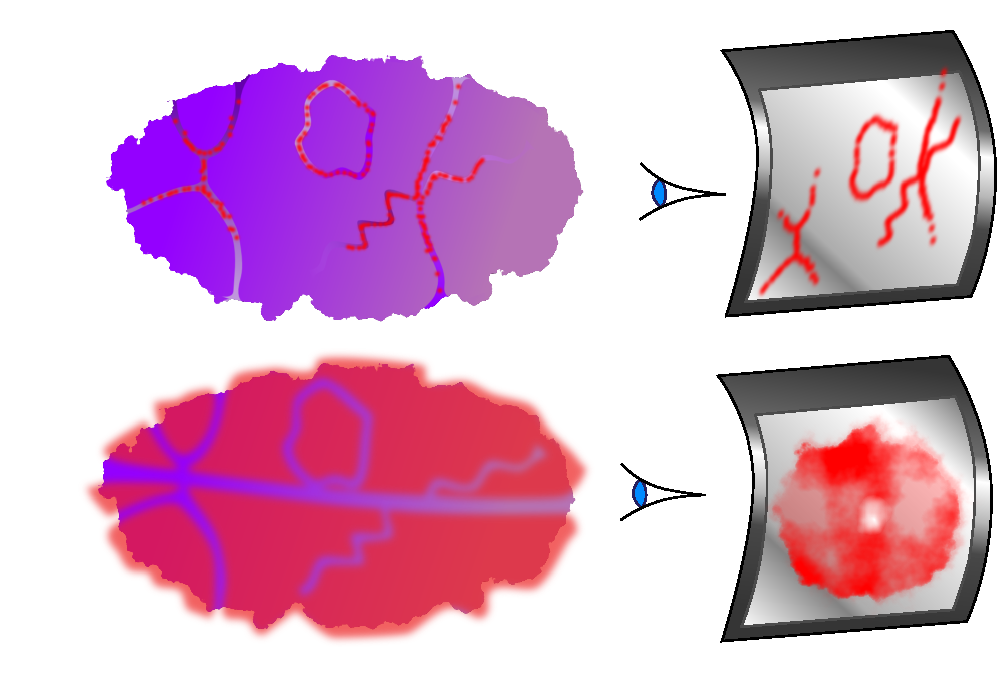
\includegraphics[width=0.6\textwidth]{figures/unsorted/side-on.pdf}
\caption{\label{fig:side-on}Fluorescence imaging of the condensate itself (bottom) makes it difficult to resolve vortices unless they are viewed end-on. The vortex cores are usually smaller than the imaging light's wavelength, and are thus also difficult to resolve unless the cloud is allowed to expand. Imaging tracer particles instead resolves both these problems.}
\end{center}
\end{figure}

If successful, this method will overcome several existing difficulties that other imaging methods face. Since vortices have previously been imaged by resonant absorption imaging of the condensate itself, they are usually viewed with the vortex line perpendicular to the image plane. If not viewed end on, the rest of the cloud obscures the low density of atoms due to the core. One solution to this problem is to slice the condensate into layers, and image them separately \cite{anderson_watching_2001}.

Our method should be able to image vortex lines side-on without destroying the condensate, since the atoms being imaged reside in the vortex core itself rather than the bulk of the condensate. This should make it possible to image the time evolution of Kelvin waves \cite{bretin_quadrupole_2003}, vortex reconnections \cite{leadbeater_sound_2001}, and vortex rings \cite{anderson_watching_2001}.

This \emph{in-situ} imaging of vortex dynamics will allow more types of vortex motion to be imaged. Dynamics of \bec s are usually imaged with a shot-by-shot method, in which repeated experiments with identical initial conditions are imaged destructively after being allowed to evolve for different amounts of time. Whilst this works for many types of dynamics, it fails for experiments that are more sensitive to initial conditions and noise (quantum or otherwise), such as turbulent flow. This includes phenomena which cannot be created reliably in the same initial state, even though the evolution thereafter would be consistent from one experimental run to the next. One such phenomenon is the spontaneous generation of vortices after evaporative cooling \cite{weiler_spontaneous_2008}.

\emph{In-situ} imaging of vortex motion has been achieved previously \cite{freilich_real-time_2010}, by ejecting a fraction of the atoms from the condensate periodically and imaging them. This process is limited by depletion of the condensate, and was also used only to image vortices end-on. The fraction of the condensate being imaged was also allowed to freely expand before being imaged, since vortex cores are otherwise unable to be resolved by the wavelength of light used. Our method requires neither free expansion or depletion of the condensate.

\subsection{Motivation: Turbulence}

It is commonly said that turbulence is one of the greatest unsolved problems of classical physics. But in what sense is it an unsolved problem? Its not a problem at all if your aim is reductionism---the Navier--Stokes equation perfectly describes the evolution of a Newtonian fluid within its domain of validity, and the process of deriving it from the underlying motion of classical particles is completely understood. It's turtles all the way down \cite[p 1]{hawking_brief_1988}; what more could we ask for?

The best comparison to make at this point, I think, is to the field of thermodynamics, for precisely the same statement can be made about the energy content and exchange between systems of particles. Thermodynamics has revealed that despite the chaotic motion of individual particles in an ensemble, definite statements can still be made about the behaviour of the system as a whole, \emph{without having to consider the dynamics of the constituent components in detail}.

This is the kind of solution people have in mind when they speak of `solving' the problem of turbulence. Laws describing the average properties of a fluid without reference to its precise flow field would not simply be interesting as describing turbulence as an emergent phenomenon, but would aid practical computations immensely, which are presently quite difficult. The flow of a turbulent fluid contains detail on such a  wide range of length scales that any finite-element analysis of a system such as say, an aeroplane wing, requires a very high resolution in order to be accurate. Following an estimate of computing power required to simulate a turbulent system down to its smallest length scales, Stanley Corrsin quipped \cite{corrsin_turbulent_1961}:
\begin{quote}
The foregoing estimate  is enough to suggest the use of analog instead of digital  computation; in particular, how about an analog consisting of a tank of water?
\end{quote}

But are we asking for too much? Perhaps the statistical properties of a turbulent fluid fundamentally cannot be decoupled from the finer details. If so, then it is wishful thinking to hope that we might do so.

However there is reason to believe that this is not the case. There are several tantalising results that hint at universal properties that all turbulent flows share, and there is the simple empirical observation that the average flow of turbulent fluids at large scales is reproducible from one experimental run to the next \cite[pp 13, 86]{davidson_turbulence:_2004}.

One of these universal results is Kolmogorov's theory of the statistics of small eddies \cite{kolmogorov_local_1941, spalding_kolmogorovs_1991}. Another is the fact that the rate of energy dissipation via the action of viscosity at small scales \emph{is independent of the viscosity itself} \cite[p 77]{davidson_turbulence:_2004}.

Then there is the Richardson energy cascade \cite{richardson_weather_2007}, in which energy is continually transferred from larger scales to smaller scales. With dissipation at the smallest scales and addition at larger scales, this allows for the existence of `steady state' turbulence.

So far I haven't mentioned superfluids at all, though a superfluid is what this project is studying. There are several interesting aspects of superfluid turbulence that differ from classical turbulence. The most obvious is the absence of viscosity;  another major difference is the quantisation of vortex lines. On scales much larger than the vortex spacing, superfluid turbulence is expected to closely resemble classical turbulence\footnote{At large scales in classical fluids, velocity gradients are small and hence viscosity can be neglected anyway.} \cite{tsubota_energy_2009}. But at smaller scales the energy dissipation mechanism is different, instead involving the production of sound waves via vortex interactions \cite{tsubota_energy_2009, vinen_how_2005}.

In certain 2\textsc{d} geometries, an \emph{inverse cascade} \cite{onsager_statistical_1949, kraichnan_inertial_1967} is predicted to take place in superfluids, whereby energy moves not from large scales to small, but from small to large, clustering quantised vortices of the same circulation direction together. This has not as of yet been observed.

To emphasise the role of vortices in turbulence in general, I will finally give a definition of turbulence, taken from \cite[p 53]{davidson_turbulence:_2004}:
\begin{quote}
Incompressible hydrodynamic turbulence is a spatially complex distribution of vorticity which advects itself in a chaotic manner in accordance with [the vorticity equation\footnote{Which is a transformation of the Navier--Stokes equation for an incompressible fluid into a form in which the vorticity field is center-stage.}]. The vorticity field is random in both space and time, and exhibits a wide and continuous distribution of length and time scales.
\end{quote}

When vorticity exists only in infinitely narrow lines, as it does in superfluid, the vorticity equation mentioned in the above definition reduces to a Biot--Savart type law which can be used to compute the motion of vortices without having to compute the entire flow field.

This is why we are interested in the study of the dynamics of quantised vortices. Unlike in classical fluids, the vortices in superfluids have a definite position and size; there is either a vortex or there is not. This may make it simpler to describe the motion of vortices statistically.

So far experimental studies of superfluid turbulence have mainly been in the context of liquid helium \cite{leggett_superfluidity_1999}; we hope to augment the existing experimental data with that obtained from \bec. The high degree of control afforded over systems of cold atoms allows the superfluid's properties to be tweaked in several ways, creating a larger parameter space in which to study turbulence than that afforded by liquid helium.

\subsection{Experiment control and analysis}

As is typical of an experimental project, much of what goes on day to day is implementation details. It's all very well to say that we want to make a turbulent condensate by pulsing some laser speckle for a few milliseconds, or that we want to ramp down a magnetic field at a certain rate, but how we achieve this in practice? First we have to set up the required equipment---a vacuum system, lasers, optics, magnetic coils, \textsc{rf} antennae. Progress on that front is detailed in section \ref{sec:experimental}.

Once the experiment is set up, we need to be able to control how the system's state changes over time. Components of the system that need to change state during an experiment are typically controlled with analogue and digital electronic signals. Shutters are opened and closed with digital edges; acousto-optical modulators shift the frequency of light passing through them according to a driving \textsc{ac} signal; and magnetic coils create field profiles depending on their current, which in turn depends on the voltage driving their control box. Once we have hardware capable of producing the required digital pulses, voltage ramps, and \textsc{ac} radio frequency signals, running an experiment comes down to programming them and having them execute their programs.

To this end we have created what is essentially a compiler, called \labscript, which takes high level instructions for what the devices should do, and generates the required low-level instructions for all the devices in an experiment, including clocking signals to keep all devices in sync. This is discussed in section \ref{sec:labscript}.

With an experimental run compiled, it needs to be programmed into, and executed on the hardware. This is performed by a program called \blacs, which also provides real-time control of the hardware when not executing pre-compiled experiments.

Experimental runs can take input parameters. For adjusting which values are to be used, and for repeating the same experiment with a range of different parameters, we have a program called \runmanager. \runmanager\ is a graphical front-end for setting these parameters and creating multi-dimensional parameter-space scans.

Two aptly named programs, \lyse\ and \bias, perform analysis of the acquired data as experiments occur. \bias\ interacts with \blacs\ in order to program the camera(s) before a run, and it performs image analysis once the run is complete. \lyse\ is a general purpose analysis system which triggers the execution of user analysis scripts whenever there is new data, computing any results and showing any plots that those scripts contain.

The software components of our control and analysis system are described in more detail in section \ref{sec:software}.
